%% PyGeoParallax-IN manuscript for Atmospheric Measurement Techniques.
%% Generated by 08_manuscript/make_amt.py from latex_source/ (the master copy); edit there.
\documentclass[amt, manuscript]{copernicus}

\usepackage{calc}
\usepackage{newunicodechar}
\newunicodechar{°}{\textdegree}
\newunicodechar{−}{\ensuremath{-}}
\newunicodechar{±}{\ensuremath{\pm}}
\newunicodechar{µ}{\textmu}
\newunicodechar{≥}{\ensuremath{\geq}}
\newunicodechar{·}{\ensuremath{\cdot}}
\newunicodechar{→}{\ensuremath{\rightarrow}}
\newunicodechar{ρ}{\ensuremath{\rho}}
\newunicodechar{×}{\ensuremath{\times}}
\providecommand{\tightlist}{\setlength{\itemsep}{0pt}\setlength{\parskip}{0pt}}
\providecommand{\passthrough}[1]{#1}

\begin{document}

\title{Parallax correction of INSAT-3DR imagery over India: an open-source tool and the limits of validation against GPM radar}

\Author[1][EMAIL-TO-BE-ADDED]{Naveen}{Bapalli}
\affil[1]{Independent researcher, India}

\runningtitle{Parallax correction of INSAT-3DR imagery over India}
\runningauthor{N. Bapalli}

\received{}
\pubdiscuss{}
\revised{}
\accepted{}
\published{}

\firstpage{1}

\maketitle

\begin{abstract}
Geostationary imagers see high clouds displaced away from the sub-satellite point. For INSAT-3DR at 74\,\textdegree\,E, deep convection over the Himalaya and Northeast India appears about 10\,km from its true position, two to three infrared pixels. We present PyGeoParallax-IN, an open-source Python tool that corrects this parallax. It estimates cloud-top height from 10.8\,\textmu m brightness temperature, traces each line of sight to the cloud top on the WGS84 ellipsoid (with terrain if a digital elevation model is given), applies a navigation correction measured from coastlines, and regrids the scene so that uncorrected and corrected datasets share one grid.

We validate the correction against GPM Ku-band radar in 63 coincident monsoon cases (2018--2024) over four Indian regions, 38 of them usable. The correction moves deep cores by 4--10\,km along the line of sight and leaves the cross-look offset unchanged. It reverses the mean storm-scale INSAT--GPM bias (from $+2.2$ to $-1.9$\,km), but the per-case improvement is not significant (18 of 30 cases). At convective cores, uncorrected INSAT cold cores already coincide with GPM deep-echo cells ($-0.1$\,km), and only about 5\,\% of the computed parallax is visible. A synthetic test confirms that the method detects parallax when it is present. A navigation correction fitted to GPM centres the cells but leaves the storm-scale agreement worse than uncorrected (Wilcoxon $p=0.027$). No single translation centres both measures, which differ by 2--5\,km. Navigation alone cannot explain this; we attribute it mainly to storm structure, and it limits GPM-based validation of absolute position to about $\pm$3--5\,km. INSAT-3DR L1C navigation errors are seasonal, 7--20\,km to the west in winter. In the cases tested, ERA5 profiles and SRTM terrain change the storm results by less than 0.5\,km. Retraining a precipitation-type U-Net on corrected instead of uncorrected input does not improve it: accuracy and macro F1 change by at most 0.12 percentage points, and convective scores fall slightly. The tool processes an India scene in 1.8\,s.
\end{abstract}

\introduction
\label{sec:introduction}

Geostationary satellites observe the Indian monsoon every 15--30 minutes and are the only source of continuous cloud and rainfall information over much of South Asia. Their images are geolocated as if every pixel lay on the Earth's surface. A cloud top several kilometres high lies on the same line of sight but closer to the satellite, so it appears displaced away from the sub-satellite point by about $h\tan(\mathrm{VZA})$, where $h$ is the cloud-top height and VZA the viewing zenith angle. This parallax displacement is zero below the satellite and grows towards the edge of the disk.

India is unusually exposed to this effect. INSAT-3DR, the operational Indian geostationary imager, sits at 74\,\textdegree\,E, close to the western edge of the country. Its viewing angle reaches 33--38\textdegree{} over the Himalaya and Northeast India, where monsoon convection reaches the tropopause at 15--17\,km. Deep convective tops there appear 8--12\,km from their true position, two to three infrared pixels. Products that use INSAT-3DR imagery, from rainfall estimates to cloud masks and machine-learning classifications of precipitation type, inherit this displacement, and comparisons with radar or rain gauges mix it with any real error.

Parallax correction is well established elsewhere. \citet{vicente2002} showed its importance for satellite rainfall estimates, and their correction has been used operationally in the GOES Hydro-Estimator since 2001 \citep{scofield2003}. \citet{bielinski2020} derived an accurate geometric solution on the ellipsoid and validated it against ground radar over Europe. Open-source corrections exist: satpy \citep{raspaud2018,satpy_parallax} assumes a spherical Earth and does not handle terrain, and pyparallax \citep{pyparallax} and JParallaxCorrect \citep{tsujino2026} work on the ellipsoid but handle neither terrain nor occlusion. For INSAT-3D, ISRO's operational Hydro-Estimator rain algorithm applies a parallax shift after \citet{vicente2002} as an internal step \citep{sac2015atbd,malhan2022}, but the step has not been documented in detail, quantified or validated. Apart from this, we found no published parallax correction, quantification of the parallax, or validation of parallax-corrected INSAT-3D or INSAT-3DR imagery against independent observations. INSAT-3D imagery has been combined with GPM radar before \citep{mishra2023}, and geostationary overshooting tops have been compared with GPM after a fixed-height parallax shift \citep{sun2024}, but whether the correction improves the agreement was not tested.

Validating a parallax correction is harder than it seems. A radar measures precipitation, not cloud top, and geolocation errors of the imager mix with the parallax. ISRO tracks INSAT geolocation error against land--sea control points: its quality-analysis system compared INSAT-3D before and after a yaw flip \citep{jindal2014}, and its data-quality reports give the error per image; for full-disk images in June 2020 it was 1.7--2.7 infrared pixels to the north \citep{mosdac_dqe2020}, comparable to the parallax itself. How the INSAT--radar offset responds to a parallax correction, and how much of the correction a radar can verify, has not been examined for India.

This paper addresses both the correction and its verification. Our contributions are:
\begin{enumerate}
  \item \textbf{An open-source tool, PyGeoParallax-IN} \citep{pygeoparallax}, designed for INSAT-3DR L1C imagery. It corrects for parallax by exact ray tracing to the cloud top on the WGS84 ellipsoid, optionally with terrain, applies a navigation correction measured from coastlines, and produces uncorrected and corrected datasets on the same grid, or on the native pixel grid, with occlusion-aware resampling. Existing open-source codes offer parts of this but not the combination.
  \item \textbf{A validation against GPM Ku-band radar}, to our knowledge the first for INSAT imagery against spaceborne radar, in 63 coincident monsoon cases (2018--2024; 38 usable) across four Indian regions that span the full range of viewing angles. It uses two independent offset measures, at the scale of the storm and of the convective core.
  \item \textbf{A test of what radar validation can resolve.} Most of the computed parallax is not visible against GPM at convective cores. With a synthetic test and a navigation correction fitted to GPM, we show that this is not a method error and cannot be explained by navigation alone, and that the two measures see different parts of the storm, which limits GPM-based validation of absolute position to about $\pm$3--5\,km. From GPM's 3-D reflectivity we measure the tilt of the convective cells and show that it is too small, towards the satellite, to hide the parallax.
  \item \textbf{A multi-year characterisation of INSAT-3DR L1C navigation error}, with a seasonal westward bias consistent with the yaw flip, and of the remaining error sources: cloud-top height (standard atmosphere versus ERA5), terrain (SRTM) and the slanted GPM radar beam.
  \item \textbf{A downstream test.} An attention U-Net for precipitation type, retrained on corrected instead of uncorrected input, does not improve. This agrees with the only earlier comparison of this kind that we know of, for SEVIRI rain rates \citep{dadderio2023}, and is the first such controlled comparison for INSAT-3DR and for precipitation type.
\end{enumerate}

Section~\ref{sec:data} describes the data, Section~\ref{sec:method} the correction method and Section~\ref{sec:validation} the validation design. Section~\ref{sec:results} presents the results, Section~\ref{sec:discussion} discusses them, and Section~\ref{sec:conclusions} concludes.

\section{Data}
\label{sec:data}
\label{sec:2}

\subsection{INSAT-3DR Imager}\label{sec:2.1}

INSAT-3DR is a geostationary satellite at 74.0° E. Its Imager scans the full disk every 30 minutes (scans start at HH:15 and HH:45) in six channels: visible (VIS, 0.65 µm), shortwave infrared (SWIR, 1.6 µm), mid-wave infrared (MIR, 3.9 µm), water vapour (WV, 6.8 µm) and two thermal infrared channels (TIR1, 10.8 µm; TIR2, 12.0 µm). The sampling interval is 1 km for VIS and SWIR and 4 km for the infrared channels at the sub-satellite point. We used the Level-1C sector product (\texttt{3RIMG\_*\_L1C\_SGP}) from MOSDAC; INSAT-3DR products use the INSAT-3D formats \citep{sac2014}. It is on a Mercator grid (\texttt{lon\_0\ =\ 75°\ E}) with pixel-centre coordinates. Calibrated counts are converted to brightness temperature (BT) or albedo through the lookup tables in each file.

The full-disk scan runs north to south, from 81° N to 81° S, in about 26.9 min (from the file start and end times). We estimate the scan time at a given latitude by linear interpolation along this sweep.

We did not use the satellite elevation and azimuth angles in the L1C files: they differ from the geometric values by about 1°. Viewing angles are computed directly (Section~\ref{sec:3.1}).

The Level-2B cloud-top pressure product (\texttt{3RIMG\_*\_L2B\_CTP}) gives cloud-top pressure and temperature in coarse boxes (about 37 km) and a clear-sky brightness temperature (CSBT) per channel. It contains no cloud-top height. We use its CSBT as the clear-sky reference for the cloud mask (Section~\ref{sec:3.2}) and its cloud-top pressure only as a cross-check. Its sub-satellite longitude attribute (82° E) is incorrect for INSAT-3DR and is ignored.

\subsection{GPM Dual-frequency Precipitation Radar}\label{sec:2.2}

GPM Core Observatory carries the Dual-frequency Precipitation Radar (DPR) \citep{hou2014}. We used the Ku-band Level-2A product (\texttt{2A.GPM.Ku}, version V08 \citep{gpm2aku_v08}; algorithm in \citet{iguchi2021}) from NASA GES DISC, full-swath (\texttt{FS}) group, about 245 km wide with a footprint of about 5 km. Variables read: storm-top height, near-surface corrected reflectivity, near-surface precipitation rate, precipitation type, bright-band height and the spacecraft position.

GPM 2A gives each footprint's position at the surface. An echo at height \(h\) lies on the slanted radar beam, displaced towards the spacecraft by about \(h\tan\theta_{\mathrm{GPM}}\), where \(\theta_{\mathrm{GPM}}\) is the local zenith angle of the beam. This displacement is up to about 5 km for a 15 km storm top at the swath edge. We place storm tops on the beam by intersecting the line from the footprint to the spacecraft with the ellipsoid surface at height \(h\), using the same Newton refinement as in Section~\ref{sec:3.3}. The median displacement in our cases is 1 km.

\subsection{Ancillary data}\label{sec:2.3}

\begin{itemize}
\tightlist
\item
  \textbf{Coastlines:} Natural Earth 10 m land polygons (public domain) \citep{naturalearth}, used for the navigation check (Section~\ref{sec:3.6}).
\item
  \textbf{Atmospheric profiles:} AFGL tropical standard atmosphere \citep{anderson1986}, 0--25 km at 1 km resolution; and ERA5 reanalysis \citep{hersbach2020,c3s2018} temperature and geopotential on 29 pressure levels (1000--50 hPa, 0.25°), at the hour nearest each case scan.
\item
  \textbf{Terrain:} SRTM GL1 \citep{farr2007}, 1 arcsecond tiles block-averaged to 0.01° (about 1 km). Heights are above the EGM96 geoid, which lies 50--105 m below the ellipsoid over India; this changes the terrain correction by under 75 m at VZA 35°, so heights are used as they are.
\end{itemize}

\subsection{Study period and regions}\label{sec:2.4}

Validation cases come from the monsoon seasons (June--September) of 2018--2024, in four regions that span the range of INSAT-3DR viewing angles over India. The navigation series (Section~\ref{sec:3.6}) covers March 2022 to December 2024.

\begin{table*}[t]
\caption{Validation regions.}\label{tab:R}
\begin{tabular}{@{}
  >{\raggedright\arraybackslash}p{(\linewidth - 4\tabcolsep) * \real{0.3333}}
  >{\raggedright\arraybackslash}p{(\linewidth - 4\tabcolsep) * \real{0.3333}}
  >{\raggedright\arraybackslash}p{(\linewidth - 4\tabcolsep) * \real{0.3333}}@{}}
\tophline
\begin{minipage}[b]{\linewidth}\raggedright
Region
\end{minipage} & \begin{minipage}[b]{\linewidth}\raggedright
Box (lat, lon)
\end{minipage} & \begin{minipage}[b]{\linewidth}\raggedright
Viewing zenith angle
\end{minipage} \\
\middlehline
South India (Kerala, Karnataka, Tamil Nadu) & 7--18° N, 73--82° E & 8--23° \\
Central India (Madhya Pradesh, Chhattisgarh) & 18--27° N, 75--86° E & 21--34° \\
Himalaya (Uttarakhand, Himachal, Nepal) & 24--33° N, 74--90° E & 28--42° \\
Northeast India and Bangladesh & 21--29° N, 88--97° E & 29--42° \\
\bottomhline
\end{tabular}
\end{table*}


% Schematic of cloud and terrain parallax (scripts/make_paper_figures.py, fig0_schematic).
\begin{figure*}[t]
  \centering
  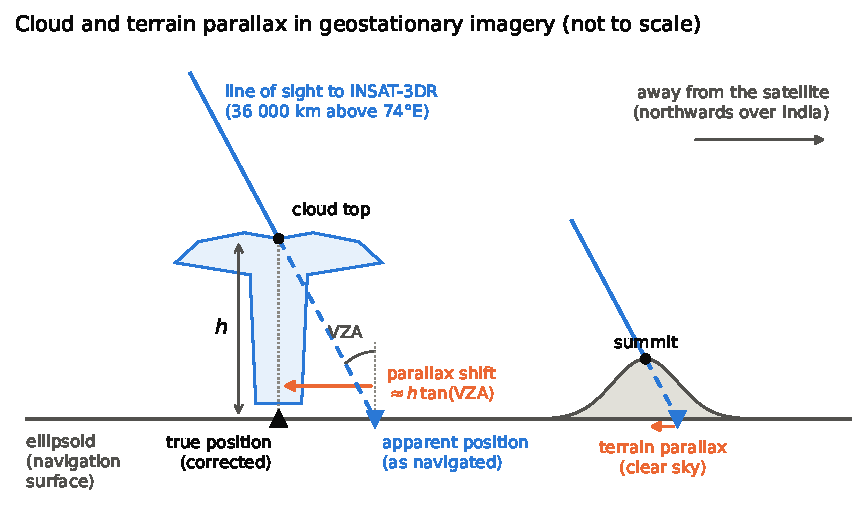
\includegraphics[width=\textwidth]{figures/fig0_schematic.pdf}
  \caption{Cloud and terrain parallax in geostationary imagery (cross-section, not to scale). A cloud top at height $h$ is seen along the line of sight from the satellite and is navigated to where that line meets the ellipsoid (apparent position), displaced away from the satellite by about $h\tan(\mathrm{VZA})$. The correction moves it back to the point on the line of sight at height $h$ (true position). Elevated terrain is displaced in the same way in clear sky.}
  \label{fig:schematic}
\end{figure*}

\section{Parallax correction method}
\label{sec:method}
\label{sec:3}

\subsection{Viewing geometry}\label{sec:3.1}

All positions are geodetic coordinates on the WGS84 ellipsoid \citep{nima2000}. A surface point at latitude \(\varphi\), longitude \(\lambda\) and ellipsoidal height \(h\) has Earth-centred, Earth-fixed (ECEF) coordinates

\[
\mathbf{p} = \begin{pmatrix} (N + h)\cos\varphi\cos\lambda \\ (N + h)\cos\varphi\sin\lambda \\ \left(N(1 - e^2) + h\right)\sin\varphi \end{pmatrix},
\qquad N = \frac{a}{\sqrt{1 - e^2\sin^2\varphi}},
\]

with semi-major axis \(a\) and eccentricity \(e\). The inverse transform uses three fixed-point iterations on latitude. Both directions agree with pyproj \citep{pyproj} to better than 1 mm.

The satellite is at \(\mathbf{s} = R_{\mathrm{geo}}(\cos\lambda_s, \sin\lambda_s, 0)\), with \(R_{\mathrm{geo}} = 42\,164\) km and \(\lambda_s = 74.0^\circ\). The unit line-of-sight vector from the ground to the satellite is \(\hat{\mathbf{d}} = (\mathbf{s} - \mathbf{p})/\lVert\mathbf{s} - \mathbf{p}\rVert\). The viewing zenith angle (VZA) is the angle between \(\hat{\mathbf{d}}\) and the local vertical; the viewing azimuth angle (VAA) comes from its east and north components. These agree with pyorbital \citep{raspaud2018} within 0.01°.

A cloud at height \(h\) appears displaced away from the satellite (Fig.~\ref{fig:schematic}) by approximately

\[
\Delta \approx h \tan(\mathrm{VZA}).
\]

Uncorrected, this displacement misplaces satellite rainfall estimates by several kilometres, especially for deep convection at high viewing angles \citep{vicente2002}. Over India the displacement is mostly northward. For a 12 km cloud top it is about 2.6 km at Kochi (VZA 12°) and 8--9 km over Northeast India and the Himalaya (VZA 34--36°).

\subsection{Cloud-top height}\label{sec:3.2}

Cloud-top height is estimated per pixel from TIR1 brightness temperature. For an opaque cloud, TIR1 BT is close to the cloud-top temperature, so the cloud-top height is the height at which the reference profile has that temperature.

\begin{enumerate}
\def\labelenumi{\arabic{enumi}.}
\tightlist
\item
  \textbf{Cloud mask.} A pixel is cloudy if its BT is more than 8 K below the ISRO clear-sky BT, sampled to the pixel by nearest neighbour. Where no clear-sky BT is available, a pixel is cloudy if BT \textless{} 270 K. Clear pixels get no height and are not moved.
\item
  \textbf{Height lookup.} BT is interpolated linearly in the AFGL tropical profile between the surface and the cold-point tropopause (17 km, 194.8 K). BT colder than the tropopause minimum, as in overshooting tops, is assigned the tropopause height.
\end{enumerate}

As an alternative, ERA5 profiles are interpolated bilinearly to each pixel, with geopotential converted to geometric height. The lookup then runs downwards from each column's cold-point tropopause (searched up to 70 hPa), so low-level inversions cannot capture high clouds. On the first 14 validation cases (2022--2024), ERA5 changes cold-core heights by −0.15 km (median) and the INSAT--GPM offsets by under 0.5 km relative to the standard atmosphere.

Profile heights are above mean sea level. We treat them as ellipsoidal heights. The difference (the geoid undulation, −50 to −100 m over India) changes the shift by less than 1\%.

The approach has known limits: semi-transparent cirrus appears warmer than its true top, so its height is underestimated; and the standard atmosphere differs from the real one by a few hundred metres.

\subsection{Ray-tracing solver}\label{sec:3.3}

The navigated (apparent) position of a pixel is where its line of sight meets the ellipsoid. A cloud at height \(h\) lies on the same line of sight, nearer the satellite. The corrected position is therefore the point

\[
\mathbf{q}(t) = \mathbf{p}_0 + t\,\hat{\mathbf{d}}
\]

on the line of sight whose geodetic height equals \(h\). Here \(\mathbf{p}_0\) is the apparent position at the navigation reference height \(h_0\) (\(h_0 = 0\) for L1C data).

We follow \citet{bielinski2020} in two steps:

\begin{enumerate}
\def\labelenumi{\arabic{enumi}.}
\tightlist
\item
  \textbf{Enlarged ellipsoid.} Intersect the line with the ellipsoid of semi-axes \(a + h\) and \(b + h\): \[
  \frac{q_x^2 + q_y^2}{(a + h)^2} + \frac{q_z^2}{(b + h)^2} = 1.
  \] This is a quadratic in \(t\), \(A t^2 + B t + C = 0\). We take the root closest to the apparent point, using the numerically stable form \(t = C/q\) or \(q/A\) with \(q = -\tfrac{1}{2}\left(B + \operatorname{sign}(B)\sqrt{B^2 - 4AC}\right)\). The enlarged ellipsoid is not a surface of constant geodetic height, but the error is only about 1 cm for a 12 km cloud over India.
\item
  \textbf{Newton refinement.} One step on the true geodetic height, \[
  t \leftarrow t + \frac{h - h_{\mathrm{geod}}(\mathbf{q}(t))}{\hat{\mathbf{d}}\cdot\hat{\mathbf{u}}(\mathbf{q}(t))},
  \] where \(\hat{\mathbf{u}}\) is the local vertical at \(\mathbf{q}\). This brings the error below 1 mm.
\end{enumerate}

Points the satellite cannot see (line of sight below the local horizon) and pixels without a height are returned as missing. The corrected position is \(\mathbf{q}(t)\) converted back to geodetic coordinates.

Unlike the spherical-Earth correction in satpy \citep{raspaud2018}, this solver works on the ellipsoid, as do two other open-source codes \citep{pyparallax,tsujino2026}, and it allows a non-zero reference height. Our solver and satpy agree within 25 m.

\subsection{Terrain}\label{sec:3.4}

Ellipsoid-navigated data misplace not only clouds but also elevated ground: over the Himalaya or the Western Ghats a 2 km ridge is displaced by about 1--1.5 km. With a digital elevation model, the solver:

\begin{itemize}
\tightlist
\item
  \textbf{cloudy pixels:} uses \(\max(h_{\mathrm{cloud}}, h_{\mathrm{ground}})\), so no cloud is placed below the ground;
\item
  \textbf{clear pixels:} moves them to where the line of sight meets the terrain (terrain parallax).
\end{itemize}

The ground height must be taken at the corrected position, which is not known in advance. We solve this by fixed-point iteration (three steps): look up the ground at the current position, correct, and repeat. The iteration converges where the terrain is less steep than the line of sight, which holds for VZA below about 70°.

With SRTM over India, the ground shift reaches 3--4 km over the Himalaya and the Tibetan Plateau, 1--2 km over the Northeast hills and under 0.5 km over the Western Ghats and Deccan. Cloud tops are far above the ground, so terrain changes the position of storm cores negligibly; in the first 14 validation cases the offsets with and without terrain are identical to 0.1 km. In clear sky, ground pixels in Himalayan scenes move by 1.3--2.5 km (median), up to about 6 km.

\subsection{Resampling onto a regular grid}\label{sec:3.5}

After correction, pixels no longer lie on a regular grid: several may land in one grid cell and some cells receive none. We resample with three rules:

\begin{enumerate}
\def\labelenumi{\arabic{enumi}.}
\tightlist
\item
  \textbf{Collisions:} when several pixels fall in one cell, the pixel with the greatest height wins. The satellite sees the highest cloud; lower ones beneath it are hidden.
\item
  \textbf{Small gaps:} cells that receive no pixel because neighbouring pixels spread apart are filled by inverse-distance weighting (power 2) from observed cells within one cell. A filled cell stays clear (no cloud-top height) if most of its neighbour weight comes from clear cells.
\item
  \textbf{Large gaps:} cells behind tall clouds, which the satellite never saw, are left empty.
\end{enumerate}

Each output cell carries a flag: 0 observed, 1 interpolated, 2 empty. Later analysis can exclude flags 1 and 2. The default grid is 0.04° (0--40° N, 60--100° E); validation uses 0.02°.

The uncorrected dataset is produced by the same resampling with the apparent positions. Both datasets therefore share exactly the same grid, which is required for the downstream model comparison.

\subsection{Navigation correction}\label{sec:3.6}

Parallax correction assumes the navigated positions are correct. We checked this by matching INSAT-3DR images to coastlines, and found errors of up to 20 km that vary with season.

\textbf{Measurement.} In each of 13 coastal windows around India, Sri Lanka, Bangladesh and Myanmar, we correlate the image with a land-fraction map. The map is made from Natural Earth polygons, blurred to the 4 km pixel footprint.

\begin{itemize}
\tightlist
\item
  \textbf{Day} (solar zenith angle \textless{} 75°): VIS albedo, using clear pixels (VIS \textless{} 30\% and TIR1 \textgreater{} 285 K).
\item
  \textbf{Night:} TIR1 with the sign reversed, since land is colder than sea, using pixels with TIR1 \textgreater{} 285 K.
\end{itemize}

A window is used only if it has at least 300 clear pixels, including at least 50 land and 50 sea pixels. Trial shifts cover ±30 km: first in 2 km steps, then in 0.5 km steps around the best value. The shift with the highest Pearson correlation \(r\) is the window's offset. Two windows whose coasts run roughly north--south or are blurred by estuaries (Chittagong, Sundarbans) measure only the east--west offset.

\textbf{Acceptance.} A window's measurement is kept only if:

\begin{itemize}
\tightlist
\item
  \(r \ge 0.6\), the best shift is not at the search edge, and both components are within 25 km;
\item
  if the window was matched in two or more scans of the same day (for example 04:15 and 06:15 UTC), they agree within 5 km in both components, and their median is used;
\item
  if it was matched in only one scan, \(r \ge 0.75\).
\end{itemize}

These rules reject matches distorted by cloud, which are common in the monsoon.

\textbf{Correction field.} Accepted window offsets are spread over the scene by inverse-distance weighting (power 2, great-circle distance, minimum distance 1 km). The north component uses only windows that measured it. The resulting east and north offsets are added to each pixel's position before cloud-top height and parallax correction.

\textbf{Seasonal behaviour.} Measurements from March 2022 to December 2024 show two states. From late September to mid-March, positions need a 7--20 km westward correction. From mid-April to September the error is small. The switch near the equinoxes is consistent with the yaw flip of the INSAT-3D-series spacecraft, a 180° rotation about the yaw axis in March and September of every year \citep{prakash2014}. ISRO's quality-analysis system compared INSAT-3D geolocation error before and after a yaw flip, using land--sea control points \citep{jindal2014}; our record extends this to several years of INSAT-3DR L1C data. During the monsoon the error is small and cannot be measured reliably for a single day: night-time matching fails because land and sea have nearly the same TIR1 temperature, and daytime matches from scans 1--2 h apart scatter by about 9--10 km. We therefore apply one correction per monsoon: the median of that year's daytime matches near the validation storms, from scans of the case days and the days before and after (2018--2024) (r ≥ 0.7, not at the search edge, both components within 25 km). The values are small, −2.0 to +3.0 km east and −0.8 to +2.5 km north. A year with fewer than 8 such matches (2018, with 2) uses the value pooled over all years, +0.5 km east and +1.5 km north. The north component is uncertain by several kilometres: different coasts give −2.5 to +8.8 km.

\subsection{Implementation}\label{sec:3.7}

The method is implemented in the open-source Python package \texttt{pygeoparallax} (v0.4.0, MIT licence; Zenodo DOI 10.5281/zenodo.23812270). The solver has a vectorised NumPy reference and a parallel Numba kernel \citep{lam2015} with identical results. The Numba kernel corrects a full disk in 0.5 s on a laptop (the NumPy version takes about 9 s); a 1-million-pixel India scene, including resampling, takes about 2 s. Unit tests (64 in v0.4.0) run on Linux and Windows under continuous integration. A command-line interface handles single scenes, parallel batches and navigation measurement.


\section{Validation design}
\label{sec:validation}
\label{sec:4}

\subsection{Case selection}\label{sec:4.1}

\begin{enumerate}
\def\labelenumi{\arabic{enumi}.}
\tightlist
\item
  \textbf{Coincident overpasses.} For every GPM orbit whose swath centre line crosses a region box between 1 June and 20 September, we estimate when the INSAT-3DR scan reaches that latitude (Section~\ref{sec:2.1}). Crossings within 5 min of an INSAT scan are kept.
\item
  \textbf{Convection screening.} Each candidate GPM file is screened for convection before INSAT data are downloaded. The densest convective cluster is found by counting GPM convective footprints in 1° bins and taking all convective footprints within about 150 km of the densest bin. A case needs at least 100 convective footprints in this cluster.
\item
  \textbf{Files per case:} the GPM 2A Ku orbit, the INSAT L1C scan nearest in time with its L2B CTP file, and daytime L1C scans of the case day and the days before and after for navigation.
\end{enumerate}

Cases were selected in two rounds: 2022--2024 for all four regions, then 2018--2021 for South and Central India, where the first round had few usable cases. In total 63 cases were processed.

\subsection{Colocation}\label{sec:4.2}

Each case is processed on a 0.02° grid over its region box. INSAT data are corrected (Section~\ref{sec:3}) and also resampled uncorrected. GPM footprints are assigned to grid cells by nearest neighbour within 3.5 km; storm tops use their slanted-beam positions (Section~\ref{sec:2.2}). Only cells inside the GPM swath are compared. Analysis is limited to within 150 km and 250 km of the centre of the densest convective cluster.

\subsection{Offset measures}\label{sec:4.3}

Because the correction is a displacement, we measure displacements directly, using two independent methods.

\textbf{Field correlation.} We find the shift of the INSAT field that best correlates with the GPM field:

\begin{itemize}
\tightlist
\item
  primary pair: \(-\)BT against GPM storm-top height (both describe storm tops);
\item
  secondary pair: \(-\)BT against near-surface reflectivity.
\end{itemize}

Integer shifts up to ±10 cells (±20 km) are tested, and the best one is refined to a fraction of a cell by fitting a parabola through the correlation at the peak and its two neighbours, separately along each axis.

\textbf{Cell cores.} Each GPM deep-echo cell (connected cells with storm top \textgreater{} 10 km, at least 8 grid cells) is paired with the INSAT cold core within 25 km of its centroid. The cold core is the centroid of pixels within 3 K of the local minimum BT. The case value is the median over its cells. This measure does not depend on the shape or extent of the anvil.

\textbf{Along and across the line of sight.} Each offset is split into a component along the line of sight (positive when INSAT must move towards the satellite to match GPM) and a component across it, using the VAA at the cluster centre. Parallax correction should change only the along-look component. The cross-look component is a control.

\textbf{Overlap scores.} We also report:

\begin{itemize}
\tightlist
\item
  intersection over union (IoU) between INSAT deep cores (BT \textless{} 220 K) and GPM deep echoes (storm top \textgreater{} 8 km);
\item
  Pearson correlation and mutual information between cold cloud (BT \textless{} 235 K) and echo (reflectivity \textgreater{} 25 dBZ).
\end{itemize}

\subsection{Usable cases}\label{sec:4.4}

A case is usable if its convective cluster has at least 100 footprints and at least one field and window gives a reliable match. A match is reliable when the best shift is inside the search range (below 9.5 cells) both before and after correction. Matches at the edge of the search usually mean the two fields describe different parts of the storm.

\subsection{Experiments}\label{sec:4.5}

Each case is run in four main states:

\begin{table*}[t]
\caption{Correction states.}\label{tab:S}
\begin{tabular}{@{}
  >{\raggedright\arraybackslash}p{(\linewidth - 4\tabcolsep) * \real{0.3333}}
  >{\raggedright\arraybackslash}p{(\linewidth - 4\tabcolsep) * \real{0.3333}}
  >{\raggedright\arraybackslash}p{(\linewidth - 4\tabcolsep) * \real{0.3333}}@{}}
\tophline
\begin{minipage}[b]{\linewidth}\raggedright
State
\end{minipage} & \begin{minipage}[b]{\linewidth}\raggedright
Navigation correction
\end{minipage} & \begin{minipage}[b]{\linewidth}\raggedright
Parallax correction
\end{minipage} \\
\middlehline
Raw & no & no \\
Coastline navigation only & per-year monsoon correction (Section~\ref{sec:3.6}) & no \\
Parallax only & no & yes \\
Coastline navigation + parallax & per-year monsoon correction & yes \\
\bottomhline
\end{tabular}
\end{table*}

Two further tests address the residual offset:

\begin{itemize}
\tightlist
\item
  \textbf{Navigation from GPM.} If the residual cell offset after parallax correction were a navigation error, a single translation fitted to it should centre both offset measures. For each case we take the median cell offset (converted to east and north) of all \emph{other} cases and apply it with parallax correction (leave one out, so no case is corrected with its own data).
\item
  \textbf{Synthetic storm.} A storm with known height and position is displaced by its computed parallax and put through the same gridding and matching code, to check that the method recovers the full parallax and zero after correction.
\end{itemize}

To separate sources of residual offset, we also compare INSAT cold-core heights with GPM maximum echo-top heights in each matched cell, and repeat the cell analysis with GPM storm tops at their surface footprints instead of on the beam.

\subsection{Sensitivity}\label{sec:4.6}

An error \(\delta h\) in cloud-top height shifts the corrected position by about \(\delta h\tan(\mathrm{VZA})\): about 0.4 km per km of height error at Mumbai and 0.7 km at Agartala. We quantify this with Monte Carlo perturbations of cloud-top height (standard deviation 1 km, 100 members) and with fixed biases of ±1 and ±2 km.

\subsection{Statistics}\label{sec:4.7}

Uncertainties are 95 \% percentile bootstrap intervals from 10 000 resamples. For the field measure, cases are resampled; for the cell measure, cases are resampled with all their cells (a cluster bootstrap), because cells of one storm are not independent. Paired comparisons between correction states use the absolute offset of each case: the median change with its bootstrap interval, the Wilcoxon signed-rank test and the exact sign test on the number of cases that improve. For the cell measure the paired test uses the per-case medians. The dependence of the raw offset on viewing angle is tested with the Spearman rank correlation and the least-squares slope against tan(VZA), with a bootstrap interval.

\subsection{Precipitation-type classification experiment}\label{sec:4.8}

To test whether the correction helps a downstream precipitation product, we retrain an existing attention U-Net for precipitation type twice: once on uncorrected input (Model A) and once on parallax-corrected input (Model B). Only the input differs between the two.

\textbf{Data.} The U-Net works on 128 × 128 tiles of the INSAT-3DR L1C Mercator grid, with four channels: TIR1, TIR2, WV and MIR. Brightness temperatures are scaled as (BT − 180 K) / 150 K and clipped to {[}0, 1{]}. Each pixel carries the GPM DPR precipitation type of the footprint matched to it. Pixels without a GPM label are ignored in the loss and in the scores. GPM positions are on the ground, so parallax displaces the input but not the labels.

\textbf{Correction.} For Model B, all tiles of a scene are mosaicked, and the grid (regular in Mercator y and in longitude) is fitted from the tile coordinates to within \(10^{-4}\) pixel. Cloud-top height comes from TIR1 with the tropical standard atmosphere, with BT \textless{} 270 K taken as cloud. Every pixel is then corrected with the solver of Section~\ref{sec:3.3} and resampled onto the original pixel grid with the occlusion-aware method of Section~\ref{sec:3.5}, before the tiles are cut out again. Cells that receive no corrected pixel (0.06 \% of labelled pixels) are filled with the nearest corrected value for the input, and their labels are dropped for both models, so A and B are scored on the same pixels. The correction moves cloud by a median of 4.4 km, about one pixel, and changes TIR1 by more than 1 K on 34 \% of pixels.

\textbf{Splits.} The training set has 5,082 patches from 823 scenes (2018 and 2021--2023); the test set has 2,197 patches from 347 scenes (September 2023 and 2024). No scene, day or GPM overpass appears in both. There is no validation split: nothing is tuned, there is no early stopping, and the test set is read only after training has finished.

\textbf{Training.} Both models use the same network (about 1.1 million parameters, with layer normalisation), class-weighted cross-entropy, the Adam optimiser at a learning rate of \(10^{-6}\), a batch size of 1 and 100 epochs. They also start from the same initial weights and see the patches in the same order (seed 42). Each model is trained once. There are three tasks:

\begin{itemize}
\tightlist
\item
  four classes: stratiform, deep convective, shallow isolated and shallow non-isolated (class weights 1, 2, 3, 3);
\item
  stratiform versus convective (1, 2.2);
\item
  rain versus no rain (1, 3).
\end{itemize}

This gives six models.

\textbf{Scores.} Scores are computed per pixel on the test set: accuracy, macro F1, and per-class F1 and critical success index, CSI = TP / (TP + FP + FN). The difference B − A is tested with a paired bootstrap over test scenes (2,000 resamples), which keeps all patches of a scene together. The two-sided p-value is taken from the bootstrap distribution of the difference.


\section{Results}
\label{sec:results}
\label{sec:5}

\subsection{Expected parallax over India}\label{sec:5.1}

The parallax shift grows with distance from the sub-satellite point at 74° E (Fig.~\ref{fig:1}). For a 12 km cloud top:

\begin{itemize}
\tightlist
\item
  about 2.5--3 km over the southern peninsula (VZA 12--15°);
\item
  5--7 km over central India (VZA 22--30°);
\item
  8--9 km over the Himalaya and Northeast India (VZA 33--38°); for a 16 km top it reaches 11--12 km there.
\end{itemize}

The shift points away from the satellite, which over India is roughly northwards; over the Northeast it turns towards the north-east (VAA up to 217°).

In the validation cases the correction moved deep convective cores (BT \textless{} 220 K) by a median of:

\begin{itemize}
\tightlist
\item
  3.9 km in South India;
\item
  7.3 km in Central India;
\item
  9.8 km over the Himalaya;
\item
  10.5 km over Northeast India.
\end{itemize}

The median over all usable cases is 7.2 km. These shifts follow tan(VZA) as expected. The solver itself agrees with pyproj, pyorbital and satpy to within 1 mm, 0.01° and 25 m respectively (Section~\ref{sec:3}).

\subsection{INSAT-3DR navigation}\label{sec:5.2}

Coastline matching shows that INSAT-3DR L1C positions carry a navigation error that changes with the season (Fig.~\ref{fig:2}). From late September to mid-March, positions need a correction of 7--20 km to the west. From mid-April to September the error is small. The switch near the equinoxes is consistent with the yaw flip of the INSAT-3D-series spacecraft, a 180° rotation about the yaw axis in March and September of every year \citep{prakash2014}.

During the monsoon the error cannot be measured reliably for a single day:

\begin{itemize}
\tightlist
\item
  Night-time matching fails because land and sea have almost the same TIR1 temperature (r \textless{} 0.4 for every night-time case scan).
\item
  Daytime matching works, but the same coast in scans 1--2 h apart differs by about 9--10 km. The best correlation is typically only 0.01--0.05 above the unshifted one.
\end{itemize}

Pooling the reliable daytime matches near the validation storms of each monsoon gives small corrections: −2.0 to +3.0 km east and −0.8 to +2.5 km north. 2018 had too few matches, so it uses the all-years value, +0.5 km east and +1.5 km north. These per-year values are used as the navigation correction.

The north component, which matters most for the parallax over India, is only weakly constrained. Individual coasts give anything from −2.5 km (Chennai) to +8.8 km (Kutch), with 5--8 km spread within one coast.

\subsection{Validation cases}\label{sec:5.3}

We processed 63 coincident INSAT--GPM cases from the monsoons of 2018--2024. GPM was within 5 min of the INSAT scan at the storm; for the usable cases the median was 1.0 min and the maximum 2.9 min.

\begin{itemize}
\tightlist
\item
  38 cases are usable (Table~\ref{tab:1}).
\item
  9 had too little convection (fewer than 100 convective footprints in the main cluster).
\item
  16 gave no reliable match in any field or window.
\end{itemize}

The usable cases span all seven years (3--7 per year). In the field measure, 30 cases give a reliable match in every correction state, and these 30 are used for paired comparisons. In the cell measure, 157--167 GPM deep-echo cells in 27--28 cases are matched to an INSAT cold core in each state.

\begin{table*}[t]
\caption{Validation cases, 2018--2024.}\label{tab:1}
\begin{tabular}{@{}
  >{\raggedright\arraybackslash}p{(\linewidth - 10\tabcolsep) * \real{0.1667}}
  >{\raggedright\arraybackslash}p{(\linewidth - 10\tabcolsep) * \real{0.1667}}
  >{\raggedleft\arraybackslash}p{(\linewidth - 10\tabcolsep) * \real{0.1667}}
  >{\raggedleft\arraybackslash}p{(\linewidth - 10\tabcolsep) * \real{0.1667}}
  >{\raggedleft\arraybackslash}p{(\linewidth - 10\tabcolsep) * \real{0.1667}}
  >{\raggedleft\arraybackslash}p{(\linewidth - 10\tabcolsep) * \real{0.1667}}@{}}
\tophline
\begin{minipage}[b]{\linewidth}\raggedright
Region
\end{minipage} & \begin{minipage}[b]{\linewidth}\raggedright
VZA at storm
\end{minipage} & \begin{minipage}[b]{\linewidth}\raggedleft
Processed
\end{minipage} & \begin{minipage}[b]{\linewidth}\raggedleft
Usable
\end{minipage} & \begin{minipage}[b]{\linewidth}\raggedleft
Too little convection
\end{minipage} & \begin{minipage}[b]{\linewidth}\raggedleft
No reliable match
\end{minipage} \\
\middlehline
South India & 9--21° & 17 & 14 & 0 & 3 \\
Central India & 22--33° & 25 & 15 & 0 & 10 \\
Himalaya & 29--37° & 11 & 4 & 6 & 1 \\
Northeast India & 31--38° & 10 & 5 & 3 & 2 \\
\textbf{Total} & & \textbf{63} & \textbf{38} & \textbf{9} & \textbf{16} \\
\bottomhline
\end{tabular}
\end{table*}

\subsection{Storm-scale offsets}\label{sec:5.4}

The correction acts only along the line of sight, as it should. The cross-look offset does not change (median change 0.0 km, 95 \% interval −0.2 to +0.2 km, 30 cases). Cross-look scatter therefore reflects storm structure, storm motion within the up to 3 min between the two observations, and the different quantities the two instruments see. It is not a parallax effect.

Along the line of sight, parallax correction reverses the mean storm-top field offset (Table~\ref{tab:2}): the mean moves from +2.2 km (95 \% interval +0.1 to +4.2 km) to −1.9 km (−4.2 to +0.3 km). The median absolute offset falls from 5.1 to 3.8 km. Case by case, however, the improvement is not significant:

\begin{itemize}
\tightlist
\item
  18 of 30 cases improve;
\item
  the median change is −1.1 km (95 \% interval −1.6 to +1.2 km);
\item
  sign test p = 0.36, Wilcoxon signed-rank p = 0.66.
\end{itemize}

Adding the per-year coastline navigation changes little: the mean is −1.0 km and the median absolute offset 4.3 km, with 17 of 30 cases better than parallax alone (p = 0.58).

\begin{table*}[t]
\caption{Mean line-of-sight offset of the storm-top field (250 km window) by region; cases valid in every state.}\label{tab:2}
\begin{tabular}{@{}
  >{\raggedright\arraybackslash}p{(\linewidth - 12\tabcolsep) * \real{0.1429}}
  >{\raggedleft\arraybackslash}p{(\linewidth - 12\tabcolsep) * \real{0.1429}}
  >{\raggedleft\arraybackslash}p{(\linewidth - 12\tabcolsep) * \real{0.1429}}
  >{\raggedleft\arraybackslash}p{(\linewidth - 12\tabcolsep) * \real{0.1429}}
  >{\raggedleft\arraybackslash}p{(\linewidth - 12\tabcolsep) * \real{0.1429}}
  >{\raggedleft\arraybackslash}p{(\linewidth - 12\tabcolsep) * \real{0.1429}}
  >{\raggedleft\arraybackslash}p{(\linewidth - 12\tabcolsep) * \real{0.1429}}@{}}
\tophline
\begin{minipage}[b]{\linewidth}\raggedright
Region
\end{minipage} & \begin{minipage}[b]{\linewidth}\raggedleft
Cases
\end{minipage} & \begin{minipage}[b]{\linewidth}\raggedleft
Mean VZA
\end{minipage} & \begin{minipage}[b]{\linewidth}\raggedleft
Applied shift at deep cores, median {[}km{]}
\end{minipage} & \begin{minipage}[b]{\linewidth}\raggedleft
Raw {[}km{]}
\end{minipage} & \begin{minipage}[b]{\linewidth}\raggedleft
Parallax {[}km{]}
\end{minipage} & \begin{minipage}[b]{\linewidth}\raggedleft
Navigation + parallax {[}km{]}
\end{minipage} \\
\middlehline
South India & 10 & 15° & 3.9 & +2.6 & +1.1 & +1.8 \\
Central India & 12 & 27° & 7.3 & +0.9 & −3.5 & −2.7 \\
Himalaya & 4 & 34° & 9.8 & +2.0 & −4.9 & −4.3 \\
Northeast India & 4 & 34° & 10.5 & +5.2 & −1.4 & +0.8 \\
\textbf{All} & \textbf{30} & & 7.2 & \textbf{+2.2} & \textbf{−1.9} & \textbf{−1.0} \\
\bottomhline
\end{tabular}
\end{table*}

Applied shifts are medians over all 38 usable cases; offsets use the 30 cases valid in every state.

\subsection{Most of the expected parallax is not visible against GPM}\label{sec:5.5}

If the uncorrected INSAT--GPM offset were pure parallax, it would equal the shift that the correction applies. It would grow from about 4 km in South India to about 10 km over the Himalaya and the Northeast. Neither measure shows this (Fig.~\ref{fig:3}).

\begin{itemize}
\tightlist
\item
  \textbf{Field measure.} The raw offset does not grow with viewing angle: Spearman ρ = −0.01, slope −0.8 km per unit tan(VZA), 95 \% interval −12.9 to +9.4 km. With 30 cases the upper bound (+9.4 km) lies just below the 10--12 km per unit tan(VZA) expected for deep convection. Against the applied shift, the fitted slope is −0.03 (Fig.~\ref{fig:3}a).
\item
  \textbf{Cell measure.} Uncorrected INSAT cold cores already sit almost on top of GPM's deep-echo cells: median −0.1 km, 95 \% interval −2.7 to +3.5 km, from a cluster bootstrap over cases. Regional medians stay within ±3 km of zero (South −2.6, Central +1.7, Himalaya −1.6, Northeast +0.4 km), and so do both periods (2018--2021 and 2022--2024). Parallax correction moves them past the cells to −4.7 km (−6.8 to −0.9 km); the per-case change is −4.5 km (p \textless{} 0.001). The median per-case ratio of raw cell offset to applied shift is 0.05 (95 \% interval −0.47 to +0.55): only about 5 \% of the computed parallax is visible. A least-squares fit of the case medians against the applied shift has a slope of +0.22 (Fig.~\ref{fig:3}b; the median of the case medians is +0.1 km).
\end{itemize}

Table~\ref{tab:3} summarises both measures in each correction state.

\begin{table*}[t]
\caption{Offsets in each correction state (30--31 cases for the field measure; 157--167 cells in 27--28 cases for the cell measure).}\label{tab:3}
\begin{tabular}{@{}
  >{\raggedright\arraybackslash}p{(\linewidth - 8\tabcolsep) * \real{0.2000}}
  >{\raggedleft\arraybackslash}p{(\linewidth - 8\tabcolsep) * \real{0.2000}}
  >{\raggedleft\arraybackslash}p{(\linewidth - 8\tabcolsep) * \real{0.2000}}
  >{\raggedleft\arraybackslash}p{(\linewidth - 8\tabcolsep) * \real{0.2000}}
  >{\raggedright\arraybackslash}p{(\linewidth - 8\tabcolsep) * \real{0.2000}}@{}}
\tophline
\begin{minipage}[b]{\linewidth}\raggedright
State
\end{minipage} & \begin{minipage}[b]{\linewidth}\raggedleft
Field mean {[}km{]}
\end{minipage} & \begin{minipage}[b]{\linewidth}\raggedleft
Field median absolute {[}km{]}
\end{minipage} & \begin{minipage}[b]{\linewidth}\raggedleft
Field cases improved vs raw
\end{minipage} & \begin{minipage}[b]{\linewidth}\raggedright
Cells, median {[}km{]} (95 \% interval)
\end{minipage} \\
\middlehline
Raw & +2.2 & 5.1 & -- & −0.1 (−2.7 \ldots{} +3.5) \\
Parallax only & −1.9 & 3.8 & 18 of 30 & −4.7 (−6.8 \ldots{} −0.9) \\
Coastline navigation + parallax & −1.0 & 4.3 & 15 of 30 & −3.3 (−5.9 \ldots{} +0.2) \\
GPM navigation + parallax (leave one out) & +4.9 & 6.0 & 10 of 31 & −0.5 (−2.6 \ldots{} +2.9) \\
\bottomhline
\end{tabular}
\end{table*}

The GPM-navigation row uses the 31 cases valid in its own states; in that set the raw field offset is +2.1 km (median absolute 4.8 km) and the parallax-only offset −1.9 km (3.7 km).

\subsection{Why the parallax is not visible}\label{sec:5.6}

We tested five explanations in turn.

\begin{enumerate}
\def\labelenumi{\arabic{enumi}.}
\item
  \textbf{The comparison method.} We put a synthetic storm with a known parallax through the same gridding and cell-matching code. The raw offset equals the full parallax: +10.9 km measured against +10.5 km expected at VZA 35°, and +3.5 against +3.9 km at VZA 15°. After correction it is about zero. Overlays of uncorrected INSAT on GPM storm tops for six high-angle cases show the same as the statistics: the cold cloud masses sit on the deep-echo cells, not 8--10 km beyond them. The method detects parallax when it is there.
\item
  \textbf{GPM's slanted beam.} Placing storm tops on the slanted Ku beam instead of at the surface footprint changes the cell medians by at most 0.6 km. This displacement has a median of 1 km and reaches 5 km. It adds scatter, not bias.
\item
  \textbf{Cloud-top height.} In 206 matched cells (29 cases) the BT-derived height of the INSAT cold core has a median of 16.6 km, and 46 \% of the cores reach the 17 km tropopause cap. The GPM maximum echo top in the same cells has a median of 11.9 km, and the median difference per cell is 3.2 km (Fig.~\ref{fig:5}). In the 14 cases of 2022--2024, ERA5 profiles instead of the standard atmosphere changed cold-core heights by −0.15 km and every offset by less than 0.5 km. The gap between infrared top and radar echo top is therefore physical: GPM's storm top is the highest range bin with echo above the Ku-band detection threshold (about 14.5--18 dBZ) \citep{hou2014,toyoshima2015}, and the small ice particles at the top of deep convection lie below it. The gap inflates the shift at the rain core by about 1--2 km. It cannot hide 4--10 km.
\item
  \textbf{Navigation.} A navigation error towards the satellite would cancel part of the parallax and shift both measures by the same amount.

  \begin{itemize}
  \tightlist
  \item
    \textbf{Coastline values.} The per-year values are only −0.8 to +2.5 km to the north.
  \item
    \textbf{ISRO's data-quality reports.} For five full-disk L1B images of 19 June 2020, measured at ground control points north-west of India, positions must move 1.7--2.7 IR pixels north and 1.0--3.3 pixels west. With 4 km IR pixels that is roughly 7--11 km north, enough to cancel most of the parallax.
  \item
    \textbf{Navigation fitted to GPM.} We tested this directly by estimating the navigation from GPM itself. Each case got the median cell offset after parallax correction of all other cases (leave one out): +5.0 km east (95 \% interval +1.4 to +5.8 km) and +5.8 km north (+2.9 to +8.7 km).
  \end{itemize}

  The GPM-fitted navigation centres the cell measure (−0.5 km) but pushes the field measure to +4.9 km and makes it worse than uncorrected (Table~\ref{tab:3}, Fig.~\ref{fig:4}):

  \begin{itemize}
  \tightlist
  \item
    median absolute offset 6.0 km;
  \item
    10 of 31 cases better than raw;
  \item
    Wilcoxon p = 0.027, sign test p = 0.07; against parallax only, p = 0.28.
  \end{itemize}

  \textbf{No single translation centres both measures.} The field and cell measures differ by 2--3 km in the raw and coastline-navigation states, and by about 5 km once the navigation is fitted to the cells. Navigation alone therefore cannot explain the result: the two measures see different parts of the storm (below). The east component of the fitted value also disagrees with ISRO's reports, which point west.
\item
  \textbf{Storm tilt.} If the cells leaned towards the satellite with height, the lean would cancel the parallax at the cell scale. GPM's 3-D reflectivity shows that they do lean, but mostly across the line of sight (Table~\ref{tab:5}). In 203 deep cells in 29 cases, the echo leans westward with height: the echo top lies 1.5 km (95 \% interval 0.6--3.1 km) and the 11--13 km layer 2.2 km west of the 2--4 km core, as expected under the upper-level easterlies of the monsoon. Towards the satellite, however, the lean is only +0.8 km (−0.9 to +1.4 km) at the echo top, because the satellite lies to the south or south-west of most cases. With other reflectivity thresholds and cell sizes this component stays between +0.4 and +0.8 km. Case by case, the median lean towards the satellite is +0.3 km, about 1 \% of the parallax that the cell measure does not see (median 6.4 km), and it does not correlate with the cell offsets (Spearman r = 0.17, p = 0.41). By region it is +1.0 km in South India, +0.9 km in Central India, +0.3 km over the Himalaya and −0.7 km in Northeast India, where a westward lean would point most directly at the satellite. The tilt of the precipitating column therefore does not hide the parallax.
\end{enumerate}

\begin{table*}[t]
\caption{Displacement of GPM Ku echo centroids from the 2--4 km convective core, median over cells with 95 \% interval (cluster bootstrap over cases). Towards the satellite is the direction of the parallax correction; the north component is within ±0.3 km of zero in every layer.}\label{tab:5}
\begin{tabular}{@{}
  >{\raggedright\arraybackslash}p{(\linewidth - 8\tabcolsep) * \real{0.1111}}
  >{\raggedright\arraybackslash}p{(\linewidth - 8\tabcolsep) * \real{0.1313}}
  >{\raggedright\arraybackslash}p{(\linewidth - 8\tabcolsep) * \real{0.2525}}
  >{\raggedright\arraybackslash}p{(\linewidth - 8\tabcolsep) * \real{0.2525}}
  >{\raggedright\arraybackslash}p{(\linewidth - 8\tabcolsep) * \real{0.2525}}@{}}
\tophline
\begin{minipage}[b]{\linewidth}\raggedright
Layer
\end{minipage} & \begin{minipage}[b]{\linewidth}\raggedright
Cells (cases)
\end{minipage} & \begin{minipage}[b]{\linewidth}\raggedright
Towards satellite {[}km{]}
\end{minipage} & \begin{minipage}[b]{\linewidth}\raggedright
East {[}km{]}
\end{minipage} & \begin{minipage}[b]{\linewidth}\raggedright
Cross-look {[}km{]}
\end{minipage} \\
\middlehline
5--7 km & 201 (29) & +0.1 (−0.1, +0.4) & −0.5 (−0.8, −0.1) & +0.3 (−0.1, +0.6) \\
8--10 km & 196 (29) & +0.3 (−0.5, +1.0) & −1.3 (−2.1, −0.8) & +1.0 (+0.4, +1.9) \\
11--13 km & 100 (26) & +0.7 (−0.6, +2.1) & −2.2 (−3.4, −0.4) & +1.9 (+0.2, +3.4) \\
Echo top & 140 (27) & +0.8 (−0.9, +1.4) & −1.5 (−3.1, −0.6) & +1.6 (+0.3, +3.1) \\
\bottomhline
\end{tabular}
\end{table*}

The two measures compare different parts of the storm. The field measure is driven by the large cold anvil against the radar's rain area, and the cell measure by the coldest tops against the tallest echoes. Their difference, 2--3 km and up to about 5 km depending on the navigation applied, is comparable to the parallax over South India and a third to a half of it at higher viewing angles. At the scale of the storm, parallax correction reverses the mean bias, and the corrected mean is not significantly different from zero. At the scale of the convective core, uncorrected cold cores already coincide with the radar cells, and correcting them with the full infrared height overshoots.

\subsection{Terrain}\label{sec:5.7}

Terrain-aware correction with SRTM moves clear-sky ground by:

\begin{itemize}
\tightlist
\item
  up to 3--4 km over the Himalaya and the Tibetan Plateau;
\item
  1--2 km over the Northeast hills;
\item
  under 0.5 km over the Western Ghats and the Deccan (Fig.~\ref{fig:6}).
\end{itemize}

In the Himalayan validation scenes, clear-sky ground pixels move by 1.3--2.5 km (median) and up to 5.8 km, and 9--19 \% of grid cells change.

At the storms (14 cases of 2022--2024), terrain makes no difference: the field and cell offsets are identical to 0.1 km with and without it. Storm tops lie 10--17 km above the ground, so the height of the ground beneath them does not enter the correction.

\subsection{Benchmark}\label{sec:5.8}

The full pipeline processed all 148 available monsoon scenes without a failure. Each scene took 1.8 s (median; 3.2 s at most) on a laptop, with about 450 MB of memory. Processing includes reading two channels over 0--40° N, 60--100° E, cloud-top height, and the corrected and uncorrected grids at 0.04°.

After correction:

\begin{itemize}
\tightlist
\item
  98.7 \% of grid cells hold an observed pixel, 1.3 \% are filled from neighbours and 0.007 \% stay empty behind tall clouds;
\item
  corrected clouds cover 2.5 \% of previously clear cells (median);
\item
  all other clear cells are identical in the corrected and uncorrected grids, so the two datasets differ only where clouds moved.
\end{itemize}

Fourteen scenes from 11--14 June 2023 turned out to be partial INSAT-3DR scans, with up to 57 \% of the image missing. The pipeline handles them. The two validation cases on those dates are unaffected because their storms lie inside the scanned part.


% Figures 1-6 (from scripts/make_paper_figures.py). Floats; LaTeX places them near Section 5.

\begin{figure*}[t]
  \centering
  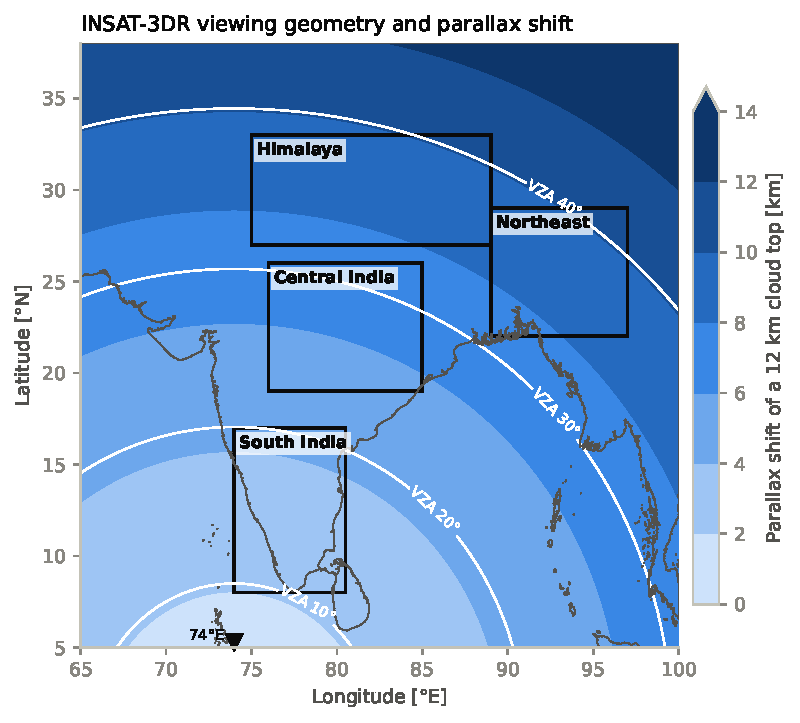
\includegraphics[width=0.8\textwidth]{figures/fig1_geometry.pdf}
  \caption{INSAT-3DR viewing geometry over South Asia. Colours: parallax shift of a 12\,km cloud top, $h\tan(\mathrm{VZA})$; white lines: viewing zenith angle. Boxes: the four validation regions. The sub-satellite point is at 74\,\textdegree\,E.}
  \label{fig:1}
\end{figure*}

\begin{figure*}[t]
  \centering
  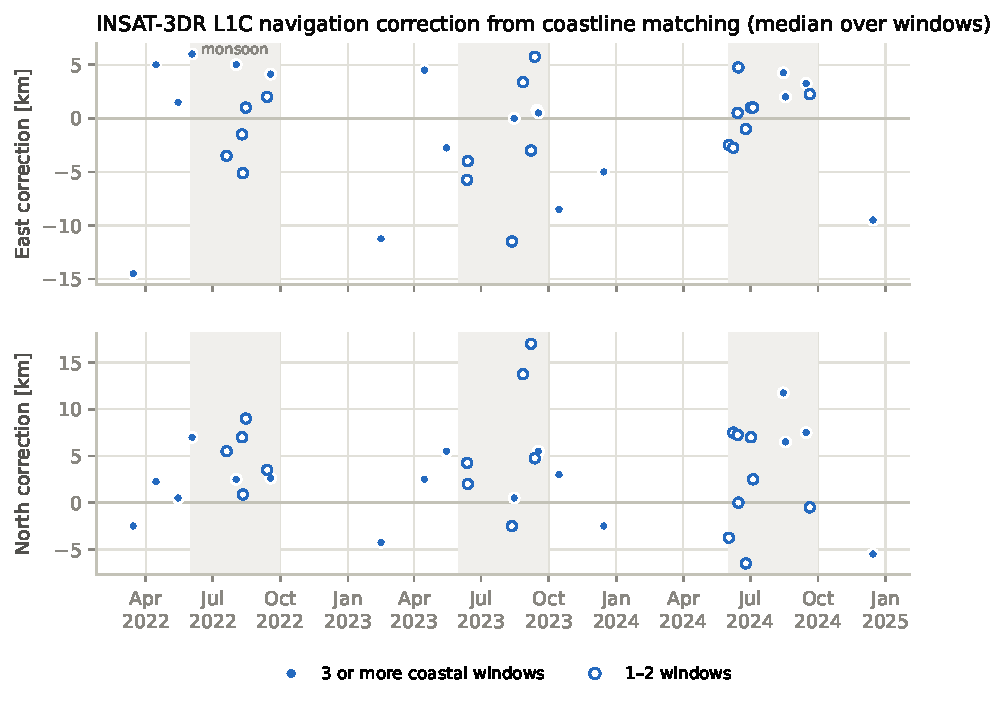
\includegraphics[width=\textwidth]{figures/fig2_navigation.pdf}
  \caption{INSAT-3DR L1C navigation correction from coastline matching, March 2022 to December 2024 (median over the accepted coastal windows of each date). Filled points: three or more windows; open points: one or two. Shading: June--September. Positive values mean INSAT positions must move east or north.}
  \label{fig:2}
\end{figure*}

\begin{figure*}[t]
  \centering
  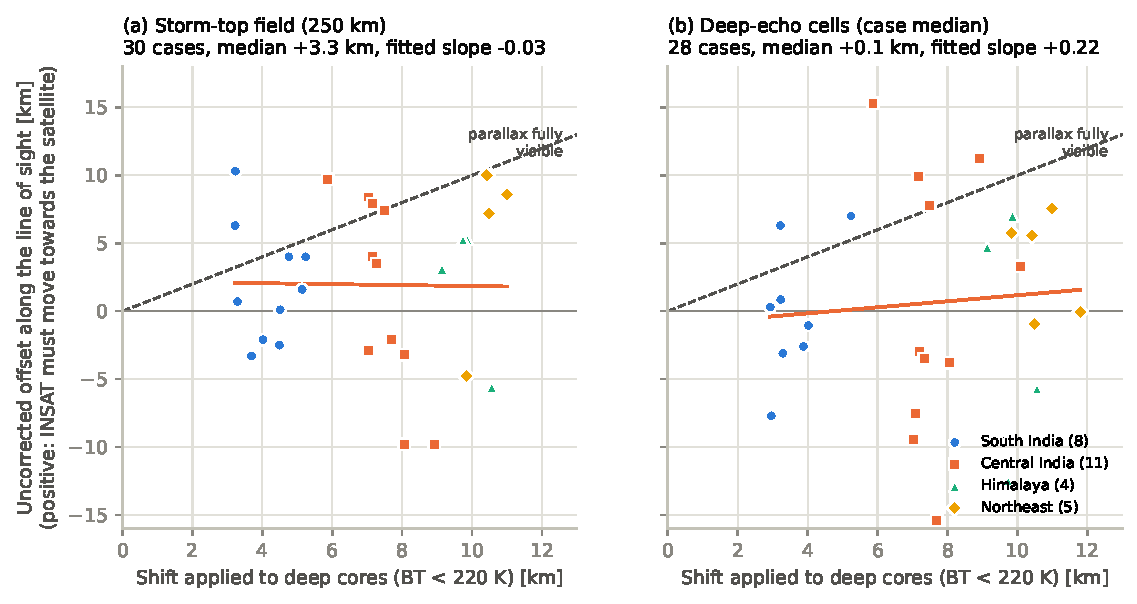
\includegraphics[width=0.9\textwidth]{figures/fig3_cases.pdf}
  \caption{How much of the computed parallax is visible against GPM. Uncorrected line-of-sight offset (GPM minus INSAT; positive: INSAT must move towards the satellite) against the shift the correction applies to deep cores in each case. (a) Storm-top field correlation, 250\,km window (30 cases); (b) median offset of the GPM deep-echo cells and their INSAT cold cores (28 cases). Dashed: parallax fully visible; orange: least-squares fit.}
  \label{fig:3}
\end{figure*}

\begin{figure*}[t]
  \centering
  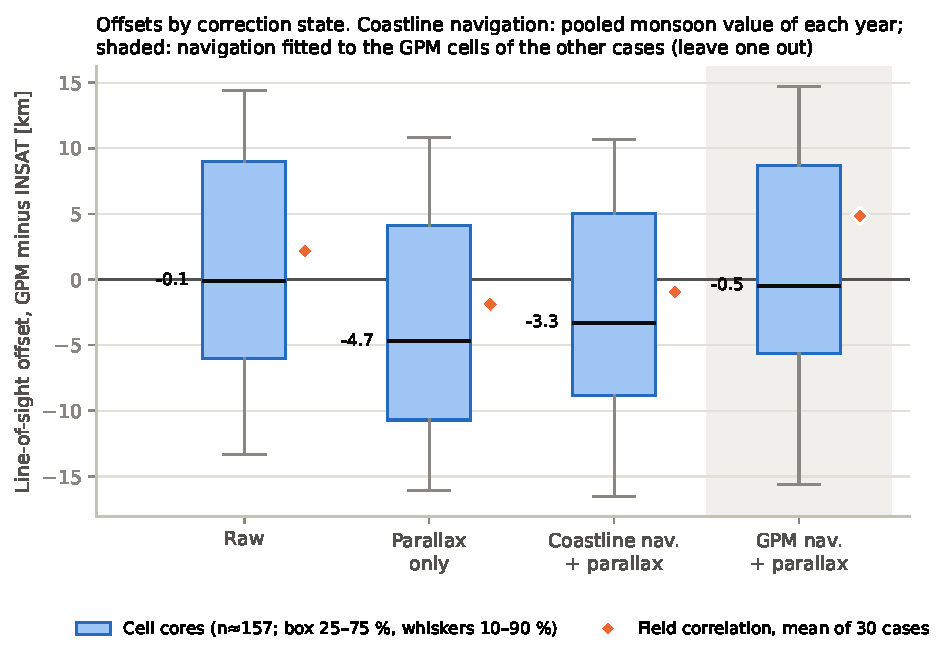
\includegraphics[width=\textwidth]{figures/fig4_states.pdf}
  \caption{Line-of-sight offsets in each correction state. Boxes: cell-by-cell offsets between GPM deep-echo cells and INSAT cold cores (box 25--75\,\%, whiskers 10--90\,\%; median labelled). Diamonds: mean field-correlation offset over 30 cases (31 for the GPM-navigation state). Coastline navigation: pooled monsoon value of each year. Shaded: navigation fitted to the GPM cells of all other cases (leave one out); it centres the cells but moves the field measure away from zero.}
  \label{fig:4}
\end{figure*}

\begin{figure*}[t]
  \centering
  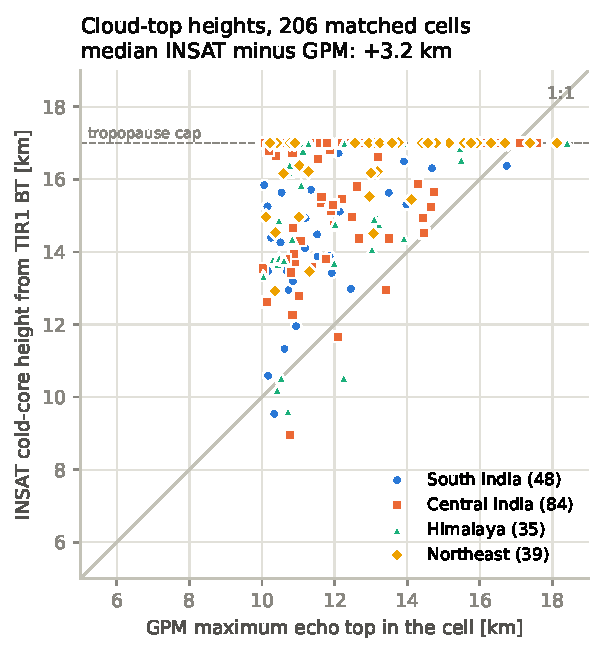
\includegraphics[width=0.6\textwidth]{figures/fig5_heights.pdf}
  \caption{Cloud-top height of the INSAT cold core (from TIR1 brightness temperature, AFGL tropical profile) against the GPM maximum echo top in the same cell, for 206 matched cells in 29 cases. Dashed line: the tropopause cap of the profile.}
  \label{fig:5}
\end{figure*}

\begin{figure*}[t]
  \centering
  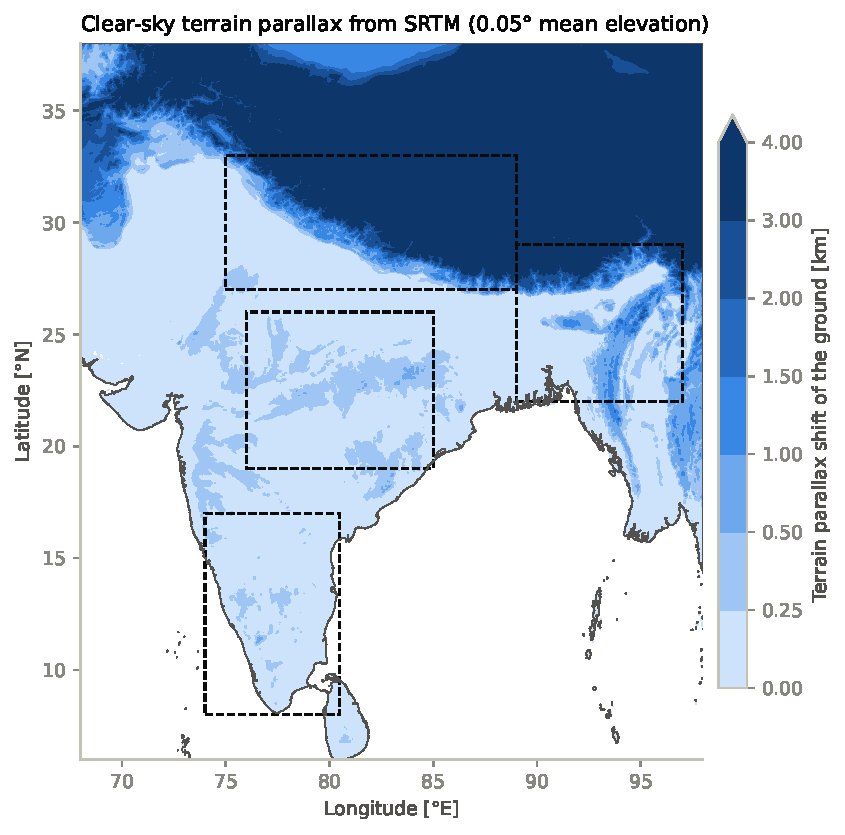
\includegraphics[width=0.8\textwidth]{figures/fig6_terrain.pdf}
  \caption{Clear-sky terrain parallax: displacement of the ground in ellipsoid-navigated INSAT-3DR imagery, from SRTM elevation averaged to 0.05\,\textdegree. Dashed boxes: validation regions.}
  \label{fig:6}
\end{figure*}

\section{Discussion}
\label{sec:discussion}
\label{sec:6}

\subsection{What the correction does, and what GPM can verify}\label{sec:6.1}

The ellipsoid ray-tracing correction is exact to well under the pixel size, and on real data it does what geometry predicts. Features move along the line of sight by h·tan(VZA), and nothing moves across it: the cross-look offset changes by a median of 0.0 km (95 \% interval −0.2 to +0.2 km). At the scale of whole storms it reverses the mean INSAT--GPM bias, from +2.2 to −1.9 km.

What GPM cannot do is confirm that the corrected positions are more accurate than the uncorrected ones. With 38 usable cases over seven monsoons:

\begin{itemize}
\tightlist
\item
  the per-case improvement in the field measure is not significant;
\item
  the cell measure says the uncorrected cores were already in place.
\end{itemize}

The two measures disagree with each other by 2--3 km, and by about 5 km once navigation is fitted to one of them, so a GPM-based validation of absolute position is limited to about ±3--5 km for monsoon deep convection. That is comparable to the parallax over South and Central India, and a third to a half of it over the Himalaya and the Northeast. The 12-case result we obtained first (10 of 12 cases improving) did not hold up in the larger sample. This is a caution for validation studies based on a few overpasses.

\subsection{Why the coldest tops and the deepest echoes coincide}\label{sec:6.2}

For the uncorrected cold cores to sit on the radar cells, the coldest infrared top of a cell must lie, on average, a parallax-sized distance towards the satellite (south) of the deep echo beneath it. We see three non-exclusive explanations:

\begin{itemize}
\tightlist
\item
  \textbf{Storm structure.} Monsoon convection over India is organised in large systems whose deep echoes reach 17 km and whose stratiform and anvil regions extend over hundreds of kilometres \citep{houze2007,romatschke2011}. The coldest top of such a system need not lie vertically above its deepest radar echo: updraft tilt in the strong easterly shear of the monsoon, and anvil spreading, could displace it by several kilometres. A systematic southward component would cancel the northward parallax. Such offsets are documented elsewhere: in a tornadic supercell the highest radar echo top lay about 10 km from the overshooting cloud top after parallax correction \citep{bluestein2019}, and across the tropics cold cloud tops cover far more area than the radar rain beneath them \citep{liu2007}. We are not aware of a measurement of this offset for monsoon storms, so it remains a hypothesis.
\item
  \textbf{Effective height.} The cold core seen at 10.8 µm is the cloud top at the tropopause (16.6 km median), about 3 km (median 3.2 km) above the radar echo top. If the radiating top of the core is spatially offset from the echo core, the full infrared height is the wrong height for matching rain.
\item
  \textbf{Navigation.} ISRO's own geolocation checks for June 2020 point to an error of 7--11 km towards the north, which would hide most of the parallax. Coastlines cannot confirm it in monsoon cloud, and fitting the navigation to GPM breaks the field measure. We cannot exclude a navigation contribution, but navigation alone cannot reconcile the two measures.
\end{itemize}

An independent geostationary view of the same storms, for example Meteosat IODC at 45.5° E, which sees the parallax in a different direction, would separate these explanations. So would ground radar at known positions. Both are left for future work.

\subsection{Navigation}\label{sec:6.3}

The INSAT-3DR L1C navigation error is seasonal: 7--20 km to the west from late September to mid-March. This is larger than the parallax, and outside the monsoon it is the dominant geolocation error. In the monsoon the coastline method gives small values (−2.0 to +3.0 km east, −0.8 to +2.5 km north per year) but cannot constrain the north component better than several kilometres, and it cannot be applied per day. Users should apply the seasonal correction outside the monsoon, and should not fit navigation to radar cells: Section~\ref{sec:5.6} shows that doing so absorbs storm structure into the navigation and degrades storm-scale agreement.

\subsection{Which cloud height to use}\label{sec:6.4}

Brightness-temperature heights put the coldest convective tops at the tropopause, a median 3.2 km above the GPM echo tops, with either the standard atmosphere or ERA5. This is mainly physical: the infrared signal comes from the top of the cloud, while the Ku-band radar detects only precipitation-sized particles, with a threshold of about 14.5--18 dBZ \citep{toyoshima2015}. The gap lies within the 2.7--5.5 km difference between cloud-top height and storm height reported from TRMM for heavy rain \citep{song2020}.

\begin{itemize}
\tightlist
\item
  For \textbf{cloud products} (cloud masks, cloud-top properties), the infrared top is the right height, and the correction places the cloud top where geometry says it is.
\item
  For \textbf{precipitation products}, the rain-relevant level lies below the infrared top, and our cell results suggest that correcting cores with the full infrared height moves the cold signal past the rain. An effective height between the echo top and the infrared top could suit precipitation better. Lower heights have helped elsewhere: correcting passive-microwave rain retrievals with the freezing level instead of the cloud-top height reduced their error against radar \citep{monsalve2026}, 40--50 \% of the cloud height worked best for parallax-only correction of irradiance \citep{wiltink2025}, and the lightning-mapper reference height was lowered from 16 to 14 km \citep{virts2020}. We are not aware of an earlier tuning of this height for geostationary infrared against spaceborne radar.
\end{itemize}

A precipitation-type classifier trained on input corrected with the full infrared height does not improve, and its convective scores fall slightly (Section~\ref{sec:6.8}).

ISRO's operational cloud-top pressure product placed deep cores 2--3 km lower than the BT heights in our first case (Kochi, 6 June 2022; r = 0.86 overall). It was not used for the correction.

\subsection{Terrain}\label{sec:6.5}

Terrain does not affect the storm results but matters for anything observed at the ground in clear sky. Over the Himalaya, ellipsoid-navigated pixels of high terrain are misplaced by several kilometres. For land-surface temperature, snow cover or surface classification in mountains, terrain-aware correction should be standard.

\subsection{Relation to earlier work}\label{sec:6.6}

\citet{vicente2002} showed that parallax and orographic corrections matter for satellite rainfall estimates from GOES. Since 2001, the GOES Hydro-Estimator \citep{scofield2003} has applied their correction operationally. \citet{bielinski2020} derived the ellipsoid solution that our solver follows; we extend it to terrain and to a navigation correction. satpy \citep{satpy_parallax} offers an open-source spherical-Earth correction for gridded geostationary data, and two open-source codes solve on the ellipsoid without terrain \citep{pyparallax,tsujino2026}. For Meteosat SEVIRI, \citet{wiltink2025} compared geometric parallax correction with an empirical shift that maximises the correlation with ground observations, the idea behind our field measure. For INSAT-3D, ISRO's Hydro-Estimator applies a parallax shift after \citet{vicente2002} before computing rain rates \citep{sac2015atbd,malhan2022}; the revised algorithm document does not describe the step \citep{varma2015}, and it has not been quantified or validated. Apart from this, we found no published parallax correction, quantification of the parallax, or validation of parallax-corrected INSAT-3D or INSAT-3DR imagery. INSAT-3D has been combined with GPM radar \citep{mishra2023}, and geostationary overshooting tops have been compared with GPM after a fixed 14 km correction \citep{sun2024}, but without testing whether the correction helps; the CloudSat/CALIPSO comparison of \citet{kotarba2026} cannot test the correction step either. To our knowledge, this study is the first evaluation of parallax correction of INSAT imagery against spaceborne radar.

Our results add a caution to radar-based validation of geostationary parallax correction. Where the expected parallax is a few kilometres, as for most of India, the measured improvement depends on which part of the storm is compared. Cell-scale comparisons can show the opposite of storm-scale ones. This agrees with reports that the benefit of geometric correction depends on the height used and on the regime \citep{wiltink2025,monsalve2026}, but we are not aware of an earlier comparison of a storm-scale and a cell-scale measure for the same storms.

Some earlier studies point the other way at the cell scale. Comparisons with ground radar have found a clear offset between the coldest satellite pixel and the radar maximum, which correction removes: over Central Europe \citep{radova2008}, over Japan, where the offset grew with colder tops across 16 events \citep{harjupa2017}, and in the single SEVIRI scene of \citet{bielinski2020}. These studies cover one or a few cases, at larger viewing angles where the parallax exceeds plausible storm-structure offsets, and mostly in mid-latitude storms. Over most of India the parallax is 4--10 km, comparable to those offsets, and monsoon systems are large and sheared, so the two results need not conflict; a multi-case test at high viewing angles would show which applies. ISRO's data-quality reports \citep{mosdac_dqe2020} already measure INSAT-3DR geolocation error per image against ground control points (for example, for 19 June 2020). Their June 2020 values point in the same northward direction as our cell result, but they are for L1B images, at control points outside the storm regions, and in one year.

\subsection{Limitations}\label{sec:6.7}

\begin{itemize}
\tightlist
\item
  \textbf{Reference instrument.} Validation uses GPM only. GPM samples each storm once, in a 245 km swath. Its echo tops differ from infrared tops by definition, and the two offset measures differ by 2--5 km depending on the navigation applied. Ground-based radar (IMD Doppler Weather Radar) at fixed sites, or a second geostationary view, would be needed to verify absolute positions to better than this.
\item
  \textbf{Sample by region.} South and Central India have 14--15 usable cases each, but the Himalaya and Northeast India only 4--5. Regional means at high viewing angles rest on few cases.
\item
  \textbf{Navigation.} The monsoon navigation correction is a per-year value whose north component is uncertain by several kilometres. The link between the seasonal change and the yaw flip rests on timing only.
\item
  \textbf{Sensitivity tests.} ERA5 profiles and SRTM terrain were tested on the 14 cases of 2022--2024 only.
\item
  \textbf{Cloud height.} Heights come from TIR1 brightness temperature. This underestimates thin cirrus, caps overshooting tops at the tropopause, and does not give the effective height relevant for precipitation.
\end{itemize}

\subsection{Effect on precipitation-type classification}\label{sec:6.8}

Section~\ref{sec:6.4} leaves open whether correcting with the infrared height helps a precipitation product. Table~\ref{tab:4} compares the U-Net trained on uncorrected input (Model A) with the same network trained on parallax-corrected input (Model B), for the three tasks of Section~\ref{sec:4.8}.

\begin{table*}[t]
\caption{Test-set scores of Model A (uncorrected input) and Model B (parallax-corrected input): 2,197 patches from 347 scenes. B − A is given with its 95 \% interval from a paired bootstrap over scenes, and p is two-sided.}\label{tab:4}
\begin{tabular}{@{}
  >{\raggedright\arraybackslash}p{(\linewidth - 12\tabcolsep) * \real{0.1566}}
  >{\raggedright\arraybackslash}p{(\linewidth - 12\tabcolsep) * \real{0.2530}}
  >{\raggedleft\arraybackslash}p{(\linewidth - 12\tabcolsep) * \real{0.0602}}
  >{\raggedleft\arraybackslash}p{(\linewidth - 12\tabcolsep) * \real{0.0602}}
  >{\raggedleft\arraybackslash}p{(\linewidth - 12\tabcolsep) * \real{0.0964}}
  >{\raggedright\arraybackslash}p{(\linewidth - 12\tabcolsep) * \real{0.3133}}
  >{\raggedleft\arraybackslash}p{(\linewidth - 12\tabcolsep) * \real{0.0602}}@{}}
\tophline
\begin{minipage}[b]{\linewidth}\raggedright
Task
\end{minipage} & \begin{minipage}[b]{\linewidth}\raggedright
Score
\end{minipage} & \begin{minipage}[b]{\linewidth}\raggedleft
A
\end{minipage} & \begin{minipage}[b]{\linewidth}\raggedleft
B
\end{minipage} & \begin{minipage}[b]{\linewidth}\raggedleft
B − A
\end{minipage} & \begin{minipage}[b]{\linewidth}\raggedright
95 \% interval
\end{minipage} & \begin{minipage}[b]{\linewidth}\raggedleft
p
\end{minipage} \\
\middlehline
Four classes & Accuracy & 0.675 & 0.674 & −0.0004 & −0.0011 to +0.0004 & 0.290 \\
& Macro F1 & 0.421 & 0.420 & −0.0012 & −0.0024 to 0.0000 & 0.050 \\
& CSI stratiform & 0.700 & 0.701 & +0.0003 & −0.0004 to +0.0012 & 0.431 \\
& CSI deep convective & 0.041 & 0.038 & −0.0030 & −0.0055 to −0.0007 & 0.008 \\
& CSI shallow isolated & 0.265 & 0.264 & −0.0006 & −0.0019 to +0.0007 & 0.388 \\
& CSI shallow non-isolated & 0.221 & 0.222 & +0.0010 & −0.0001 to +0.0020 & 0.070 \\
Stratiform / convective & Accuracy & 0.709 & 0.709 & +0.0000 & −0.0012 to +0.0013 & 0.920 \\
& Macro F1 & 0.686 & 0.685 & −0.0004 & −0.0014 to +0.0007 & 0.494 \\
& CSI stratiform & 0.628 & 0.628 & +0.0006 & −0.0010 to +0.0022 & 0.481 \\
& CSI convective & 0.429 & 0.428 & −0.0012 & −0.0023 to −0.0001 & 0.039 \\
Rain / no rain & Accuracy & 0.863 & 0.863 & +0.0001 & −0.0002 to +0.0005 & 0.412 \\
& Macro F1 & 0.718 & 0.717 & −0.0002 & −0.0007 to +0.0002 & 0.329 \\
& CSI rain & 0.347 & 0.346 & −0.0005 & −0.0012 to +0.0001 & 0.120 \\
\bottomhline
\end{tabular}
\end{table*}

Correcting the input does not improve the classifier. In all three tasks, accuracy and macro F1 of Model B are within 0.0012 of Model A. Only the convective classes change consistently, and they get slightly worse:

\begin{itemize}
\tightlist
\item
  deep convective CSI falls from 0.041 to 0.038 (B − A = −0.0030, 95 \% interval −0.0055 to −0.0007, p = 0.008);
\item
  convective CSI in the stratiform/convective task falls from 0.429 to 0.428 (−0.0012, −0.0023 to −0.0001, p = 0.039);
\item
  four-class macro F1 falls by 0.0012 (p = 0.05).
\end{itemize}

Stratiform scores and rain detection do not change significantly.

Three points qualify this result:

\begin{itemize}
\tightlist
\item
  \textbf{Size.} The changes are small. The largest relative change, 7 \% of deep convective CSI, is in a class that the network barely detects with either input (F1 0.08).
\item
  \textbf{Multiple tests.} With 22 scores tested, one or two p-values below 0.05 are expected by chance. None would pass a Bonferroni correction (p \textless{} 0.002).
\item
  \textbf{One run per model.} Each model was trained once, and run-to-run variation (for example from non-deterministic GPU operations) was not measured. It may be of similar size.
\end{itemize}

The result agrees with the only earlier comparison of this kind that we know of: a SEVIRI U-Net for rain rate, trained against GPM, also performed better without parallax correction \citep{dadderio2023}. Networks can learn a consistent displacement on their own \citep{hilburn2021}, so a geometric pre-correction adds little and brings its own errors (cloud-top height, holes and duplicates at occlusions).

The pattern is nevertheless consistent with Section~\ref{sec:5.5}. Uncorrected cold cores already sit on the GPM convective cells, so moving them by the full infrared parallax pulls the cold signal away from the convective labels, and convective scores drop slightly. Stratiform rain is horizontally extensive and insensitive to a one-pixel shift. For this classifier, correcting with the full infrared height brings no benefit. An effective height closer to the radar echo top (Section~\ref{sec:6.4}) can be tested with the same set-up.


\conclusions
\label{sec:conclusions}

We have presented PyGeoParallax-IN, an open-source tool that corrects INSAT-3DR imagery for cloud parallax. It uses exact ray tracing on the WGS84 ellipsoid, with optional terrain and a navigation correction measured from coastlines. We tested it against GPM radar in 38 usable monsoon cases from 2018--2024.

\begin{enumerate}
  \item \textbf{The correction is exact and behaves as geometry predicts.} It agrees with independent implementations to within millimetres to tens of metres. It moves features only along the line of sight, and it moves deep convection by 4\,km over South India and about 10\,km over the Himalaya and Northeast India.
  \item \textbf{At storm scale it reverses the mean bias, but GPM cannot show a per-case gain.} The mean INSAT--GPM offset of the storm-top field moves from $+2.2$ to $-1.9$\,km, not significantly different from zero. Only 18 of 30 cases improve, which is not significant.
  \item \textbf{At convective cores, most of the computed parallax is not visible.} Uncorrected INSAT cold cores already coincide with GPM deep-echo cells ($-0.1$\,km), and correction moves them about 5\,km past ($p<0.001$). Only about 5\,\% of the computed parallax is visible. A synthetic test shows that the method recovers the full parallax when it is present.
  \item \textbf{Navigation alone cannot explain the result.} A navigation correction fitted to the GPM cells centres the cell measure but leaves the storm-scale agreement worse than uncorrected. No single translation centres both measures, which differ by 2--5\,km depending on the navigation applied. We attribute this mainly to storm structure: the coldest infrared tops and the deepest radar echoes are different targets. It limits GPM-based validation of absolute position to about $\pm$3--5\,km, comparable to the parallax over most of India.
  \item \textbf{Navigation, cloud height and terrain.}
  \begin{itemize}
    \item INSAT-3DR L1C navigation errors are seasonal, 7--20\,km to the west from late September to mid-March, consistent with the yaw flip. In the monsoon they are small and cannot be measured per day from coastlines.
    \item Brightness-temperature heights of the coldest tops lie at the tropopause, about 3\,km above the GPM echo tops, with either the standard atmosphere or ERA5.
    \item In the 14 cases of 2022--2024, ERA5 profiles change the offsets by less than 0.5\,km and terrain by less than 0.1\,km; terrain moves clear-sky ground in the Himalaya by up to 6\,km.
  \end{itemize}
  \item \textbf{Correcting the input does not improve a precipitation-type classifier.} A U-Net retrained on corrected input scores the same as on uncorrected input in three tasks (accuracy and macro F1 within 0.12 percentage points). Its convective scores fall slightly (deep convective CSI from 0.041 to 0.038), consistent with item 3 and with an earlier SEVIRI study in which the uncorrected network also performed better \citep{dadderio2023}; the changes are small and come from one training run per model.
  \item \textbf{The tool is fast and ready for downstream use.} It processes an India scene in 1.8\,s and writes uncorrected and corrected datasets that are identical in clear sky.
\end{enumerate}

For cloud products, the infrared cloud-top height is the right one, and the correction places cloud tops where geometry says they are. For precipitation applications, the rain-relevant level lies below the infrared top. For a precipitation-type U-Net, correcting with the infrared height brought no benefit. An effective height closer to the radar echo top, now an option in the tool, is the natural next test. Verifying absolute positions to better than a few kilometres will need ground radar at known sites or a second geostationary view. Users should not fit navigation corrections to radar cells. The code, scripts and validation case lists are available at \url{https://github.com/bapallinaveen60/PyGeoParallax-IN}.


\codeavailability{PyGeoParallax-IN (version 0.4.0, MIT licence), with the scripts, case lists and U-Net training and comparison scripts used in this study, is archived on Zenodo \citep{pygeoparallax}: \url{https://doi.org/10.5281/zenodo.23812270}. The concept DOI \url{https://doi.org/10.5281/zenodo.23666957} always resolves to the latest version. Development continues at \url{https://github.com/bapallinaveen60/PyGeoParallax-IN}.}

\dataavailability{INSAT-3DR Imager L1C and L2B products are available from MOSDAC, Space Applications Centre, ISRO (\url{https://www.mosdac.gov.in}) after free registration. GPM DPR 2A Ku version 8 data are available from NASA GES DISC \citep{gpm2aku_v08}. ERA5 pressure-level data are available from the Copernicus Climate Data Store \citep{c3s2018}. SRTM elevation data \citep{farr2007} were obtained through OpenTopography, and coastlines from Natural Earth \citep{naturalearth}. The validation case list (GPM orbits and INSAT scan times) is part of the code archive.}

\authorcontribution{NB designed the study, wrote the software, carried out the validation and the U-Net experiments, and wrote the manuscript.}

\competinginterests{The author has declared that there are no competing interests.}

\begin{acknowledgements}
INSAT-3D and INSAT-3DR data were provided by the Meteorological and Oceanographic Satellite Data Archival Centre (MOSDAC), Space Applications Centre, ISRO. GPM data were provided by the NASA/JAXA Global Precipitation Measurement mission through the NASA Goddard Earth Sciences Data and Information Services Center (GES DISC). ERA5 was produced by the European Centre for Medium-Range Weather Forecasts (ECMWF) and made available by the Copernicus Climate Change Service. SRTM data were provided by NASA and USGS through OpenTopography, and coastlines by Natural Earth. The software builds on NumPy, SciPy, xarray, pyproj, Numba, h5py and TensorFlow; satpy and pyorbital were used for independent checks. The author thanks the developers of the attention U-Net and of the labelled INSAT--GPM patches used in Sect.~\ref{sec:4.8}. An AI assistant (Claude, Anthropic) was used to help write code and edit the text; the author reviewed all of it and takes full responsibility for the content. This research received no external funding.
\end{acknowledgements}

\bibliographystyle{copernicus}
\bibliography{references}

\end{document}
